% 附录 U：聚变增益 Q、自加热与点火（v1.18.0 新增）
% 数值唯一来源：tools/calc/appU_calc.py -> tools/calc/appU_calc.txt（正文数字的唯一来源；检查项 P24）
% 时间单位写成 s/ms，避免中文字符进入数学字体；全部数字可用仓库脚本复算。
% 版权口径：只借鉴经典教材与文献的物理结论、公式形式与题型；文字、数值与表格自拟并独立复算。
% 本书不列 DOI，只给书名、作者、年份、卷期页。
% 本附录与附录 S、附录 T 共用同一组三个工作点；P 的口径差异在 U.3 显式声明。

\section{Q 是什么：三个能量账本}
\label{sec:app-u-ledger}

第 10 章讲过 Lawson 判据与三重积，附录 S 把约束写成一个数 $\tau_E$。但工程上最先被问到的
问题不是"能不能点着"，而是"投进去一份加热功率，能换回几份聚变功率"。这个比值就是增益
$Q$。本附录把 $Q$ 拆成三本能量账，看它怎样决定自加热、点火与电厂的账。

\begin{equation}
Q \equiv \frac{P_{\mathrm{fus}}}{P_{\mathrm{aux}}}
\label{eq:app-u-q}
\end{equation}

三个账本分别是：

\begin{itemize}
  \item \textbf{账本一（外部投入）}：$P_{\mathrm{aux}}$ 是从电网或储能系统送进等离子体的加热
        功率，微波、中性束、射频都算在这里。它是"花钱"的那一项。
  \item \textbf{账本二（聚变产出）}：D-T 反应放出 $17.6\ \mathrm{MeV}$，其中 $3.5\ \mathrm{MeV}$
        归 $\alpha$ 粒子（留在等离子体里继续加热），$14.1\ \mathrm{MeV}$ 归中子（穿出等离子体
        去包层）。于是 $P_{\mathrm{fus}}$ 一分为二：
\end{itemize}

\begin{equation}
P_\alpha = \frac{1}{5}P_{\mathrm{fus}}, \qquad
P_{\mathrm{n}} = \frac{4}{5}P_{\mathrm{fus}}
\label{eq:app-u-split}
\end{equation}

\begin{itemize}
  \item \textbf{账本三（能量损失）}：等离子体通过输运把能量漏到壁上，稳态下漏掉的必须补回来，
        即 $P_{\mathrm{loss}} = W/\tau_E$。这一项决定温度能停在哪儿。
\end{itemize}

聚变功率本身由反应率决定。D-T 等离子体里氘氚各占一半（$n_{\mathrm D}=n_{\mathrm T}=n/2$，
$n$ 为总离子密度），反应率密度为 $(n^2/4)\langle\sigma v\rangle$，于是

\begin{equation}
P_{\mathrm{fus}} = \frac{n^2}{4}\,\langle\sigma v\rangle_{\mathrm{DT}}\,E_{\mathrm{fus}}\,V,
\qquad
\langle\sigma v\rangle_{\mathrm{DT}} \approx 1.1\times10^{-24}\,T^2\ \ \mathrm{m^3/s}
\label{eq:app-u-pfus}
\end{equation}

其中 $T$ 以 keV 计，$E_{\mathrm{fus}} = 17.6\ \mathrm{MeV} = 2.819831\times10^{-12}\ \mathrm{J}$，
$V$ 是等离子体体积。$\langle\sigma v\rangle$ 用第 10 章卡片上的两参数拟合：它在
$10\ \mathrm{keV}$ 附近给出 $1.1\times10^{-22}\ \mathrm{m^3/s}$，与 Bosch-Hale 数据相符；
但 $T<5\ \mathrm{keV}$ 时这个拟合会高估约 2 倍，本附录所有低温行只当趋势看，绝对值不可当真。

把附录 S 表 S.2 的三个工作点代进式 \eqref{eq:app-u-q} 与式 \eqref{eq:app-u-pfus}，
得到表 \ref{tab:app-u-accounts}。$\tau_E$、$T$、$W$ 三列与附录 S 逐字一致——两个附录用的是
同一组输入、同一套 IPB98(y,2) 口径。

\begin{table}[htbp]
\centering
\small
\begin{tabular}{@{}p{3.2cm}p{1.8cm}p{1.8cm}p{1.6cm}p{1.7cm}p{1.8cm}p{1.6cm}@{}}
\toprule
装置 & $P_{\mathrm{aux}}$ [MW] & $\tau_E$ [s] & $T$ [keV] & $W$ [MJ] & $P_{\mathrm{fus}}$ [MW] & $Q$ \\
\midrule
D1 ITER 量级    & 150.0 & 2.4762 & 9.194 & 371.4 & 556.5 & 3.710 \\
D2 JET 量级     & 15.0  & 0.3827 & 2.336 & 5.7   & 0.9   & 0.058 \\
D3 DIII-D 量级  & 10.0  & 0.1055 & 1.649 & 1.1   & 0.1   & 0.014 \\
\bottomrule
\end{tabular}
\caption{三个工作点的增益 $Q$。$P_{\mathrm{aux}}$ 为外部加热功率，与附录 S 表 S.2 的
$P$ 是同一个量（口径差别见 U.3）。}
\label{tab:app-u-accounts}
\end{table}

D1 一行的细节值得拆开看：$P_{\mathrm{fus}}=556.5\ \mathrm{MW}$ 中，
$P_\alpha = 111.3\ \mathrm{MW}$ 留在等离子体里，$P_{\mathrm{n}} = 445.2\ \mathrm{MW}$ 去包层；
按 $V=832.2\ \mathrm{m^3}$ 摊开，$\alpha$ 加热的功率密度是 $1.337\times10^{5}\ \mathrm{W/m^3}$。
D2、D3 的 $Q$ 只有 $0.058$ 与 $0.014$，不是装置"差"，而是温度太低：$T=2.336$ 与
$1.649\ \mathrm{keV}$ 时 $\langle\sigma v\rangle \propto T^2$ 给出的反应率比 D1 小两个量级，
聚变功率自然只有 $0.9$ 与 $0.1\ \mathrm{MW}$。

\begin{tip}{Q 的四个语义节点}{tip-app-u-ledger}
$Q=1$ 叫\textbf{得失相当}（breakeven）：聚变功率刚好等于外部加热功率，但注意这时的
$\alpha$ 加热只占 $1/6$，等离子体仍靠外部加热维持。$Q=5$ 时 $\alpha$ 加热与外部加热各占
一半，是"燃烧等离子体"的门槛。$Q=10$ 是 ITER 的设计目标：$500\ \mathrm{MW}$ 聚变功率、
$50\ \mathrm{MW}$ 加热功率。$Q\to\infty$（外部加热可以关掉）才叫\textbf{点火}。四个节点
对应四件不同的事，混用就会出现"Q=1 就自持了"这类错误。
\end{tip}

{\footnotesize
\textbf{出处：} $Q$ 的定义与四个语义节点参照 Wesson《Tokamaks》第 4 版（Oxford, 2011）
第 1 章，以及 Freidberg《Plasma Physics and Fusion Energy》（Cambridge, 2007）第 5、13 章。
D-T 反应能与 $\alpha$/中子 $1:4$ 的功率分配见本书第 10 章。三个工作点由附录 S 的
IPB98(y,2) 口径独立复算，未复制任何教材表格数值。
}

\section{$\alpha$ 加热份额：一个只依赖 Q 的数}
\label{sec:app-u-falpha}

自加热占多大比例，是判断"能不能少开一点外部加热"的依据。由式 \eqref{eq:app-u-q} 与
式 \eqref{eq:app-u-split}，$P_\alpha = QP_{\mathrm{aux}}/5$，于是

\begin{equation}
f_\alpha \equiv \frac{P_\alpha}{P_\alpha + P_{\mathrm{aux}}}
= \frac{QP_{\mathrm{aux}}/5}{QP_{\mathrm{aux}}/5 + P_{\mathrm{aux}}}
= \frac{Q}{Q+5} = \frac{1}{1+5/Q}
\label{eq:app-u-falpha}
\end{equation}

这个式子的形式值得记住：$f_\alpha$ 只与 $Q$ 有关，不含 $n$、$T$、$\tau_E$、装置尺寸。
也就是说，一旦知道一台装置的 $Q$，自加热份额就定了，与它多大、多强无关。
表 \ref{tab:app-u-falpha} 给出几个节点的值。

\begin{table}[htbp]
\centering
\small
\begin{tabular}{@{}p{1.6cm}p{1.8cm}p{9.0cm}@{}}
\toprule
$Q$ & $f_\alpha$ & 含义 \\
\midrule
1      & 0.1667 & 得失相当：$\alpha$ 加热只占六分之一，外部加热仍是主体 \\
2      & 0.2857 & 外部加热仍占七成以上 \\
3.710  & 0.4259 & 附录 S 的 D1 外部加热点（本书基准） \\
5      & 0.5000 & $\alpha$ 加热与外部加热各占一半，燃烧等离子体门槛 \\
10     & 0.6667 & ITER 设计点：三分之二的加热来自聚变自身 \\
20     & 0.8000 & 自加热占八成，外部加热主要用来控制剖面 \\
50     & 0.9091 & 已接近点火 \\
$\infty$ & 1.0000 & 点火：外部加热可以关掉 \\
\bottomrule
\end{tabular}
\caption{自加热份额 $f_\alpha = Q/(Q+5)$。$Q$ 只有 $1$ 时，把外部加热关掉会立刻熄火——
这正是"得失相当"与"点火"必须分开讲的原因。}
\label{tab:app-u-falpha}
\end{table}

两个反直觉之处。第一，$Q=1$ 听起来像"够了"，但此时 $f_\alpha$ 只有 $1/6$，外部加热一停，
$P_{\mathrm{loss}}$ 里六分之五的来源消失，温度会迅速掉下去。第二，$f_\alpha$ 增长得比想象
慢：从 $Q=10$ 提到 $Q=20$，自加热份额只从 $0.6667$ 升到 $0.8000$，代价却是把
$P_{\mathrm{fus}}$ 与等离子体参数同时推高一大截。

\begin{tip}{为什么门槛是 Q=5 而不是 Q=1}{tip-app-u-loop2}
把 $Q=5$ 代进式 \eqref{eq:app-u-falpha} 得 $f_\alpha=0.5$：自加热与外部加热等量。再往下
提高 $Q$，自加热占优，外部加热逐渐退居"控制手段"（控制剖面、抑制不稳定性、驱动电流）。
所以聚变界把 $Q\ge5$ 作为燃烧等离子体的门槛，而把 $Q=1$ 只当作一个能量收支的记号。
\end{tip}

{\footnotesize
\textbf{出处：} $\alpha$ 加热份额的表达式由本节自行推导（只用 $P_\alpha=P_{\mathrm{fus}}/5$
与 $Q$ 的定义）。
物理背景参照 Wesson《Tokamaks》第 4 版第 1 章与 ITER Physics Basis
（1999, \textit{Nucl. Fusion} \textbf{39}）。表 \ref{tab:app-u-falpha} 的数值由
\texttt{tools/\allowbreak{}calc/\allowbreak{}appU\_calc.py} 算出。
}

\section{自加热闭环：迭代找不动点}
\label{sec:app-u-loop}

上面的 $Q$ 是"加热功率给定"的算法：先定 $P_{\mathrm{aux}}$，再由 $\tau_E$ 定 $T$，最后算
$P_{\mathrm{fus}}$。但聚变一旦发生，$\alpha$ 粒子会把功率加回等离子体，$P_{\mathrm{loss}}$
里就多了一项。稳态时

\begin{equation}
P_{\mathrm{loss}} = P_{\mathrm{aux}} + P_\alpha = \frac{W}{\tau_E},
\qquad W = 3nTV
\label{eq:app-u-balance}
\end{equation}

而 $\tau_E$ 自己又依赖于总加热功率——附录 S 的 IPB98(y,2) 定标律里 $P$ 的指数是 $-0.69$：

\begin{equation}
\tau_E = \tau_E^{\mathrm{IPB98}}\!\left(P_{\mathrm{tot}}\right),
\qquad P_{\mathrm{tot}} \equiv P_{\mathrm{aux}} + P_\alpha
\label{eq:app-u-ipb}
\end{equation}

两个式子互相咬住，只能迭代：

\begin{equation}
P_{\mathrm{tot}}^{(k+1)} = P_{\mathrm{aux}}
+ \frac{1}{5}P_{\mathrm{fus}}\!\left(T^{(k)}\right),
\qquad
T^{(k)} = \frac{\tau_E\!\left(P_{\mathrm{tot}}^{(k)}\right)P_{\mathrm{tot}}^{(k)}}{3nV}
\label{eq:app-u-loop}
\end{equation}

从 $P_{\mathrm{tot}}^{(1)}=P_{\mathrm{aux}}=150\ \mathrm{MW}$ 起手，D1 的迭代轨迹如表
\ref{tab:app-u-iter}。

\begin{table}[htbp]
\centering
\small
\begin{tabular}{@{}p{1.2cm}p{2.0cm}p{1.9cm}p{1.7cm}p{2.0cm}p{1.8cm}p{1.5cm}@{}}
\toprule
步 & $P_{\mathrm{tot}}$ [MW] & $\tau_E$ [s] & $T$ [keV] & $P_{\mathrm{fus}}$ [MW] & $P_\alpha$ [MW] & $Q$ \\
\midrule
1  & 150.00 & 2.4762 & 9.194  & 556.45 & 111.29 & 3.710 \\
2  & 261.29 & 1.6884 & 10.920 & 785.00 & 157.00 & 5.233 \\
3  & 307.00 & 1.5107 & 11.480 & 867.52 & 173.50 & 5.783 \\
4  & 323.50 & 1.4571 & 11.667 & 896.14 & 179.23 & 5.974 \\
5  & 329.23 & 1.4395 & 11.731 & 905.94 & 181.19 & 6.040 \\
8  & 332.08 & 1.4310 & 11.762 & 910.81 & 182.16 & 6.072 \\
12 & 332.20 & 1.4306 & 11.764 & 911.00 & 182.20 & 6.073 \\
\bottomrule
\end{tabular}
\caption{D1 的自加热闭环迭代。第 11、12 步之间 $P_{\mathrm{tot}}$ 只差 $0.003\ \mathrm{MW}$，
已经收敛；收敛点 $Q=6.073$ 高于表 \ref{tab:app-u-accounts} 的 $3.710$，原因见正文。}
\label{tab:app-u-iter}
\end{table}

收敛点是 $P_{\mathrm{tot}}=332.2\ \mathrm{MW}$、$\tau_E=1.4306\ \mathrm{s}$、
$T=11.764\ \mathrm{keV}$、$P_{\mathrm{fus}}=911.0\ \mathrm{MW}$、
$P_\alpha=182.2\ \mathrm{MW}$、$Q=6.073$。

注意这里出现的两个口径，混起来就会算出矛盾的数字：
\begin{itemize}
  \item \textbf{口径一（附录 S 与表 \ref{tab:app-u-accounts}）}：$P$ 取\textbf{外部加热功率}
        $P_{\mathrm{aux}}$。它回答"给定加热系统，能得到多少聚变功率"，三个装置都停在这一步，
        所以 D1 的 $Q=3.710$。
  \item \textbf{口径二（本节迭代）}：$P$ 取\textbf{总加热功率}
        $P_{\mathrm{tot}}=P_{\mathrm{aux}}+P_\alpha$。它把自加热算进功率平衡，温度因此抬高
        （$9.194\to11.764\ \mathrm{keV}$），$P_{\mathrm{fus}}$ 也抬高
        （$556.5\to911.0\ \mathrm{MW}$），于是 $Q$ 升到 $6.073$。
\end{itemize}
两个数都对，但必须说清是哪一个口径。本书约定：报装置工作点时用口径一（与附录 S 一致），
讨论自加热与点火时用口径二。

为什么迭代一定收敛，而不是"越烧越热"？把两个指数串起来看。由 IPB98(y,2) 的
$P^{-0.69}$ 与 $W=3nTV=\tau_E P_{\mathrm{tot}}$ 可得

\begin{equation}
T \propto \frac{\tau_E P_{\mathrm{tot}}}{nV} \propto P_{\mathrm{tot}}^{\,1-0.69}
= P_{\mathrm{tot}}^{\,0.31},
\qquad\text{于是}\qquad
P_\alpha \propto T^2 \propto P_{\mathrm{tot}}^{\,0.62} < 1
\label{eq:app-u-gain}
\end{equation}

$0.62<1$ 是说：总功率涨 $1\%$，自加热只涨 $0.62\%$，追不上。这条反馈的回路增益小于 1，
不动点存在且稳定——$\alpha$ 自加热是\textbf{自稳的负反馈}，不是热失控。数值上可以验证：
$P_{\mathrm{tot}}=100$、$150$、$225\ \mathrm{MW}$ 三点给出的
$T/P_{\mathrm{tot}}^{0.31}$ 恒为 $1.94496$；由迭代第 2、4 步反解
$\diff\ln T/\diff\ln P_{\mathrm{tot}} = 0.3100$，与解析值 $0.31$ 一致。

\begin{tip}{把闭环画成一条折线}{tip-app-u-loop}
在 $(P_{\mathrm{tot}}, P_\alpha)$ 平面上画两条线：一条是"供给线"
$P_\alpha = QP_{\mathrm{aux}}/5$（斜率为正的直线），一条是"需求线"
$P_\alpha \propto P_{\mathrm{tot}}^{0.62}$（斜率小于 1 的幂函数）。两条线的交点就是不动点。
若指数大于 1（需求线更"陡"），交点会变成不稳定平衡，温度一路上冲——真实等离子体之所以
可控，正因为定标律给出的指数小于 1。
\end{tip}

{\footnotesize
\textbf{出处：} 功率平衡与 $W=3nTV$ 的写法与附录 S 第 S.1、S.4 节一致。
IPB98(y,2) 定标律
及其 $P^{-0.69}$ 指数取自附录 S 式 (S.6) 一带的同一口径（原式源自 ITER Physics Basis,
1999, \textit{Nucl. Fusion} \textbf{39}）。迭代格式、收敛性与指数 $0.62$ 的推导为本书自拟，
数值由 \texttt{tools/\allowbreak{}calc/\allowbreak{}appU\_calc.py} 复算。
}

\begin{figure}[htbp]
\centering
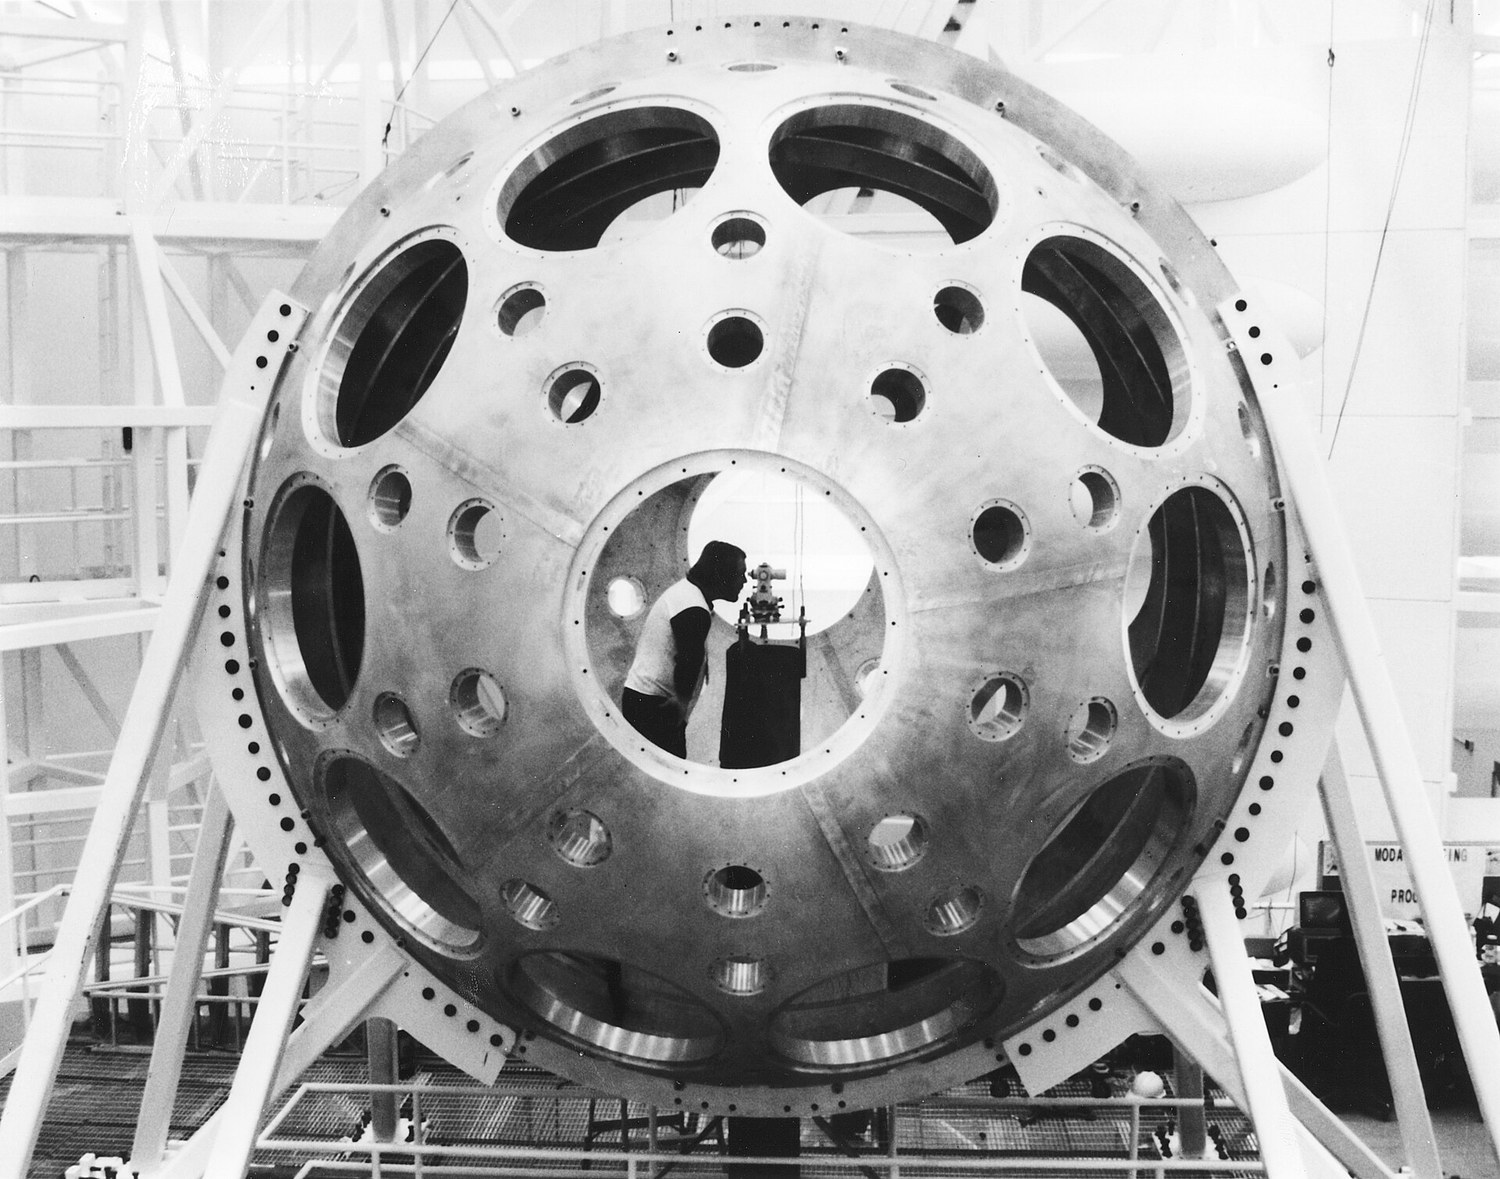
\includegraphics[width=0.72\textwidth]{../figures/u_nova_chamber.jpg}
\caption{NOVA 靶室：点火这条路最早的十束激光平台。本节的三重积阈值不是纸面条件，它对应的是一间十米级的靶室和几十束激光。}
\label{fig:photo-appu2}
\figsource{LLNL，Public domain（Wikimedia Commons）}
\end{figure}

\section{点火：三重积阈值与 Greenwald 极限的夹击}
\label{sec:app-u-ignition}

点火的定义是外部加热可以关掉，即 $\alpha$ 加热单独撑住全部损失：

\begin{equation}
P_\alpha = P_{\mathrm{loss}}
\label{eq:app-u-ignition}
\end{equation}

把 $P_\alpha = P_{\mathrm{fus}}/5$、$P_{\mathrm{fus}} = (n^2/4)\langle\sigma v\rangle E_{\mathrm{fus}}V$
与 $P_{\mathrm{loss}} = 3nTV/\tau_E$ 代进去，$V$ 与小括号一路消掉，只剩

\begin{equation}
n\tau_E = \frac{60\,T_{\mathrm J}}{\langle\sigma v\rangle E_{\mathrm{fus}}}
\label{eq:app-u-ntau}
\end{equation}

其中 $T_{\mathrm J}$ 是把 $T$ 换成焦耳后的值。再把式 \eqref{eq:app-u-pfus} 的
$\langle\sigma v\rangle \approx 1.1\times10^{-24}T^2$ 代入，$T$ 也消掉了：

\begin{equation}
nT\tau_E > 3.0992\times10^{21}\ \mathrm{keV\,s\,m^{-3}}
\label{eq:app-u-triple}
\end{equation}

这个结果有两层意思。第一层是有用的：点火条件可以用一个乘积来记，量级约
$3\times10^{21}$ $\mathrm{keV\,s\,m^{-3}}$，与教科书常引的数字一致。第二层必须声明：
\textbf{$T$ 被消掉是 $\langle\sigma v\rangle \propto T^2$ 这个拟合的产物}。真实反应率在
$15\ \mathrm{keV}$ 附近有一个极小值（Bosch-Hale 曲线），所以在低温端与高温端门槛会抬高，
不会像式 \eqref{eq:app-u-triple} 那样与 $T$ 完全无关。表 \ref{tab:app-u-triple} 列出几个温度
上的 $n\tau_E$ 要求，可以看出低温端要求更高。

\begin{table}[htbp]
\centering
\small
\begin{tabular}{@{}p{2.0cm}p{5.0cm}p{5.2cm}@{}}
\toprule
$T$ [keV] & 点火所需 $n\tau_E$ [$\mathrm{m^{-3}\,s}$] & 说明 \\
\midrule
5.0  & $6.1983\times10^{20}$ & 低温端 $\langle\sigma v\rangle\propto T^2$ 使要求偏高 \\
8.0  & $3.8740\times10^{20}$ & \\
10.0 & $3.0992\times10^{20}$ & 本书 $\langle\sigma v\rangle$ 拟合的"甜点"附近 \\
15.0 & $2.0661\times10^{20}$ & 真实曲线在此处最有利 \\
20.0 & $1.5496\times10^{20}$ & \\
\bottomrule
\end{tabular}
\caption{点火所需的 $n\tau_E$。乘积 $nT\tau_E$ 在本节的拟合下恒为
$3.0992\times10^{21}\ \mathrm{keV\,s\,m^{-3}}$，所以 $n\tau_E$ 与 $T$ 成反比。}
\label{tab:app-u-triple}
\end{table}

现在把 D1 放进去。在 $T=9.194\ \mathrm{keV}$ 上，点火要求
$n\tau_E = 3.3709\times10^{20}\ \mathrm{m^{-3}\,s}$，而 D1 实有
$nT\tau_E = 2.299\times10^{21}\ \mathrm{keV\,s\,m^{-3}}$，是阈值的 $74.2\%$——
已经不远，但还差一截。D2 只有 $1.2\%$，D3 只有 $0.3\%$，都差两个量级。

那么差的这一截能不能靠"多加点燃料"补上？逐条算：
\begin{itemize}
  \item 在同 $T$、同 $\tau_E$ 下点火需把 $n_{19}$ 从 $10.100$ 提到 $13.613$
        （$\times1.3478$），对应 $P_\alpha$ 从 $111.3$ 升到 $150.0\ \mathrm{MW}$、
        $P_{\mathrm{fus}}$ 从 $556.5$ 升到 $750.0\ \mathrm{MW}$。
  \item 若改用 $P_{\mathrm{fus}}\propto n^2$ 粗估（密度升、温度不变），只需
        $n_{19}\times\sqrt{750.0/556.5} = \times1.1610$，即 $n_{19}=11.726$。
  \item 但密度上限由 Greenwald 极限给出：$n_G = I_p/(\pi a^2) = 1.1937\times10^{20}\ \mathrm{m^{-3}}$，
        D1 工作点已经用到 $84.6\%$。按第一种算法，点火需要 $n/n_G = 982.3\%$，
        即 Greenwald 极限的 $9.8$ 倍。
\end{itemize}

这就是托卡马克的困境：三重积与密度极限从两侧夹住工作空间，D1 量级的装置够不到点火。
所以 ITER 把目标定在 $Q=10$（而不是"点火"）：既能验证自加热主导的燃烧等离子体物理，
又不要求突破密度极限。工程上更实用的路径是提高 $\tau_E$（H 模、台基、更大尺寸）而不是
硬堆密度。

{\footnotesize
\textbf{出处：} 点火条件 $P_\alpha=P_{\mathrm{loss}}$、三重积形式的推导与 Greenwald 极限的
引用遵循 Lawson (1957) \textit{Proc. Phys. Soc. B} \textbf{70}, 6 与 Freidberg
《Plasma Physics and Fusion Energy》第 13 章。
反应率拟合与 $E_{\mathrm{fus}}$ 见第 10 章
与 Bosch \& Hale (1992) \textit{Nucl. Fusion} \textbf{32}, 611。Greenwald 极限公式与
$n_G$ 的数值取自本书附录 M 第 M.5 节（口径一致）。全部数字由 \texttt{tools/\allowbreak{}calc/\allowbreak{}appU\_calc.py}
复算。
}

\section{工程增益：Q 单独不是好指标}
\label{sec:app-u-qeng}

\begin{equation}
Q \propto P_{\mathrm{aux}}^{\,-0.38}
\label{eq:app-u-qaux}
\end{equation}

上式来自把两个指数相乘：$T\propto P_{\mathrm{aux}}^{0.31}$（IPB98 的 $P^{-0.69}$），
$P_{\mathrm{fus}}\propto T^2\propto P_{\mathrm{aux}}^{0.62}$，于是
$Q = P_{\mathrm{fus}}/P_{\mathrm{aux}} \propto P_{\mathrm{aux}}^{-0.38}$。
\textbf{它随外部加热功率单调下降}——加热加得越猛，$Q$ 越难看。表 \ref{tab:app-u-qaux}
是固定 D1 的 $n$、$B$、$I_p$ 后扫 $P_{\mathrm{aux}}$ 的结果。

\begin{table}[htbp]
\centering
\small
\begin{tabular}{@{}p{2.0cm}p{1.8cm}p{1.7cm}p{1.7cm}p{2.0cm}p{1.6cm}@{}}
\toprule
$P_{\mathrm{aux}}$ [MW] & $\tau_E$ [s] & $T$ [keV] & $W$ [MJ] & $P_{\mathrm{fus}}$ [MW] & $Q$ \\
\midrule
150.0 & 2.4762  & 9.194 & 371.4 & 556.5 & 3.710 \\
100.0 & 3.2756  & 8.108 & 327.6 & 432.8 & 4.328 \\
50.0  & 5.2845  & 6.540 & 264.2 & 281.6 & 5.632 \\
20.0  & 9.9445  & 4.923 & 198.9 & 159.5 & 7.977 \\
10.0  & 16.0433 & 3.971 & 160.4 & 103.8 & 10.381 \\
5.0   & 25.8825 & 3.203 & 129.4 & 67.5  & 13.510 \\
\bottomrule
\end{tabular}
\caption{固定 D1 的 $n$、$B$、$I_p$，只改外部加热功率。$Q$ 随 $P_{\mathrm{aux}}$ 上升而下降，
而 $P_{\mathrm{fus}}$ 恰好相反。$T<5\ \mathrm{keV}$ 的行受 $\langle\sigma v\rangle\propto T^2$
高估影响（约 2 倍），只看趋势。}
\label{tab:app-u-qaux}
\end{table}

这张表藏着一个陷阱。若只盯 $Q$，会得到"$P_{\mathrm{aux}}$ 越小越好"的结论：要在 D1 上做出
$Q=10$，只需 $P_{\mathrm{aux}} = 11.035\ \mathrm{MW}$——听起来比 ITER 的 $50\ \mathrm{MW}$
还厉害。但同一行给出 $\tau_E = 14.9894\ \mathrm{s}$、$T = 4.094\ \mathrm{keV}$、
$P_{\mathrm{fus}} = 110.3\ \mathrm{MW}$：这是一台"加热很省、聚变功率也很小"的装置，
$110\ \mathrm{MW}$ 的聚变功率离电厂差得远。所以 $Q$ 必须与 $P_{\mathrm{fus}}$（或最终的电功率）
一起看，单看 $Q$ 会被"少加热"刷出来的高值骗过去。

这就引出工程增益。把电厂的热与电连起来（教学简化：只计加热功率，忽略电流驱动、包层增殖、
泵循环与占空比）：

\begin{equation}
Q_{\mathrm{eng}} \equiv \frac{P_e}{P_{\mathrm{grid}}}
= \frac{\eta_{\mathrm{th}}\left(P_{\mathrm{fus}}+P_{\mathrm{aux}}\right)}{P_{\mathrm{aux}}/\eta_{\mathrm{aux}}}
= \eta_{\mathrm{th}}\eta_{\mathrm{aux}}\left(Q+1\right)
\label{eq:app-u-qeng}
\end{equation}

其中 $P_{\mathrm{th}} = P_{\mathrm{fus}}+P_{\mathrm{aux}}$ 是热功率，$P_e = \eta_{\mathrm{th}}P_{\mathrm{th}}$
是电功率，$P_{\mathrm{grid}} = P_{\mathrm{aux}}/\eta_{\mathrm{aux}}$ 是从电网取来的功率
（加热系统自身有效率损失）。令 $Q_{\mathrm{eng}}=1$ 得

\begin{equation}
Q_{\mathrm{eng}} = 1 \quad\Longleftrightarrow\quad
Q = \frac{1}{\eta_{\mathrm{th}}\eta_{\mathrm{aux}}} - 1 = 5.250
\label{eq:app-u-qeng1}
\end{equation}

取 $\eta_{\mathrm{th}} = \eta_{\mathrm{aux}} = 0.40$，表 \ref{tab:app-u-qeng} 给出三个代表点的
完整工程账。

\begin{table}[htbp]
\centering
\small
\begin{tabular}{@{}p{2.8cm}p{1.6cm}p{1.5cm}p{1.6cm}p{1.6cm}p{1.6cm}p{1.5cm}@{}}
\toprule
工作点 & $P_{\mathrm{fus}}$ [MW] & $P_{\mathrm{aux}}$ [MW] & $P_{\mathrm{th}}$ [MW] & $P_e$ [MW] & $P_{\mathrm{grid}}$ [MW] & $Q_{\mathrm{eng}}$ \\
\midrule
D1 外部加热点    & 556.5 & 150.0 & 706.5  & 282.6 & 375.0 & 0.754 \\
自加热闭环点     & 911.0 & 150.0 & 1061.0 & 424.4 & 375.0 & 1.132 \\
ITER 设计点      & 500.0 & 50.0  & 550.0  & 220.0 & 125.0 & 1.760 \\
\bottomrule
\end{tabular}
\caption{工程增益（教学简化：$\eta_{\mathrm{th}}=\eta_{\mathrm{aux}}=0.40$，只计加热功率）。
第一行是本书基准点：$Q=3.710$ 时 $Q_{\mathrm{eng}}=0.754<1$，电厂净输出为负。}
\label{tab:app-u-qeng}
\end{table}

三点结论。第一，$Q=3.710$ 的 D1 外部加热点 $Q_{\mathrm{eng}}=0.754$：聚变是"做出来了"，
但电厂账还是亏的。第二，$Q_{\mathrm{eng}}$ 的盈亏平衡在 $Q=5.250$，比"得失相当"的 $Q=1$
高得多——差在热效率与加热效率两个 $0.40$ 上。第三，ITER 设计点 $Q=10$ 对应
$Q_{\mathrm{eng}}=1.760$，这才是"聚变电站"意义上的正增益。教学简化必须标明：真实电厂账还要
减掉电流驱动功率、包层与氚循环的功耗、以及占空比造成的停机时间。

{\footnotesize
\textbf{出处：} $Q$ 随 $P_{\mathrm{aux}}$ 下降的指数关系由本节用 IPB98(y,2) 的指数自行推导。
工程增益的写法参照 Freidberg《Plasma Physics and Fusion Energy》第 13 章与 ITER Physics
Basis（1999, \textit{Nucl. Fusion} \textbf{39}）中关于再循环功率的讨论，简化为
$\eta_{\mathrm{th}}\eta_{\mathrm{aux}}(Q+1)$ 并已在正文标明教学简化。数值由
\texttt{tools/\allowbreak{}calc/\allowbreak{}appU\_calc.py} 复算。
}

\section{六道估算练习}
\label{sec:app-u-problems}

\textbf{练习 1（$\alpha$ 加热份额）}
D1 外部加热点的 $Q=3.710$，求 $f_\alpha$；若做到 $Q=10$ 呢？再解释为什么 $Q=1$ 时
$\alpha$ 加热只占六分之一。

\textbf{解答}：直接代入式 \eqref{eq:app-u-falpha}。$Q=3.710$ 给
$f_\alpha = 3.710/8.710 = 0.4259$；$Q=10$ 给 $10/15 = 0.6667$。
$Q=1$ 时 $P_{\mathrm{fus}} = P_{\mathrm{aux}}$，于是
$P_\alpha = P_{\mathrm{aux}}/5 = 0.2P_{\mathrm{aux}}$，
$f_\alpha = 0.2/(1+0.2) = 1/6 = 0.1667$——外部加热仍是八成以上的来源，
关掉就熄火。这也说明"得失相当"与"自持"是两件事。

\textbf{练习 2（中子功率与第一壁负载）}
D1 的 $P_{\mathrm{fus}} = 556.5\ \mathrm{MW}$，其中 $4/5$ 是中子功率。若第一壁面积取
$800\ \mathrm{m^2}$，平均中子壁负载是多少？

\textbf{解答}：$P_{\mathrm{n}} = 0.8\times556.5 = 445.2\ \mathrm{MW}$；
$445.2/800 = 0.5565\ \mathrm{MW/m^2}$。这个数要记住量级：中子壁负载是包层与冷却设计的
硬约束，与 $\alpha$ 加热（留在芯部）走的是两条完全不同的路。

\textbf{练习 3（自加热闭环）}
从 $P_{\mathrm{tot}} = 150\ \mathrm{MW}$ 起手，按式 \eqref{eq:app-u-loop} 迭代三步，
列出 $P_{\mathrm{tot}}$ 与 $Q$，并说明为什么第四步之后变化就很小了。

\textbf{解答}：三步给出 $P_{\mathrm{tot}} = 150.0 \to 261.3 \to 307.0\ \mathrm{MW}$，
对应 $Q = 3.710 \to 5.233 \to 5.783$（完整轨迹见表 \ref{tab:app-u-iter}）。
变化越来越小的原因是回路增益小于 1：$T\propto P_{\mathrm{tot}}^{0.31}$，
$P_\alpha\propto T^2\propto P_{\mathrm{tot}}^{0.62}$，每迭代一次的"修正量"按
$0.62$ 的幂衰减，所以收敛是几何式的。若指数大于 1，温度就会一路上冲。

\textbf{练习 4（点火三重积）}
由 $P_\alpha = P_{\mathrm{loss}}$ 与 $\langle\sigma v\rangle \approx 1.1\times10^{-24}T^2$
推出 $nT\tau_E$ 的点火阈值；再算 D1 达到了阈值的百分之几。

\textbf{解答}：把三个表达式代入并消去 $V$，得
$n\tau_E = 60T_{\mathrm J}/(\langle\sigma v\rangle E_{\mathrm{fus}})$；
代入反应率拟合后 $T$ 消掉，$nT\tau_E > 3.0992\times10^{21}\ \mathrm{keV\,s\,m^{-3}}$。
D1：$n_{19}=10.1$、$T=9.194\ \mathrm{keV}$、$\tau_E=2.4762\ \mathrm{s}$，得
$nT\tau_E = 2.2994\times10^{21}$，是阈值的 $74.2\%$。
提醒：阈值与 $T$ 无关是 $T^2$ 拟合的产物，真实曲线在 $15\ \mathrm{keV}$ 附近更有利。

\textbf{练习 5（Q=10 的陷阱）}
固定 D1 的 $n$、$B$、$I_p$，要让 $Q=10$ 需要多大的 $P_{\mathrm{aux}}$？此时
$P_{\mathrm{fus}}$ 与 $T$ 是多少？这说明单看 $Q$ 有什么问题？

\textbf{解答}：解 $Q=10$ 得 $P_{\mathrm{aux}} = 11.03\ \mathrm{MW}$、
$\tau_E = 14.99\ \mathrm{s}$、$T = 4.09\ \mathrm{keV}$，但
$P_{\mathrm{fus}}$ 只有 $110.3\ \mathrm{MW}$。$Q$ 高是因为分母（外部加热）被压小了，
而不是因为产出大；这样的"装置"没有电厂的影子。所以 $Q$ 必须与 $P_{\mathrm{fus}}$ 或
工程增益 $Q_{\mathrm{eng}}$ 一起报。另外 $T<5\ \mathrm{keV}$ 时
$\langle\sigma v\rangle\propto T^2$ 会高估约 2 倍，这一行只看趋势。

\textbf{练习 6（工程增益）}
取 $\eta_{\mathrm{th}} = \eta_{\mathrm{aux}} = 0.40$，求 $Q=3.710$ 与 $Q=10$ 的
$Q_{\mathrm{eng}}$，以及 $Q_{\mathrm{eng}}=1$ 对应的阈值 $Q$。

\textbf{解答}：由式 \eqref{eq:app-u-qeng}，$Q=3.710$ 给
$Q_{\mathrm{eng}} = 0.4\times0.4\times4.710 = 0.754$；$Q=10$ 给
$0.16\times11 = 1.760$。阈值由式 \eqref{eq:app-u-qeng1}：
$Q = 1/0.16 - 1 = 5.250$。结论：要让聚变在电厂账上为正，$Q$ 要到 $5$ 以上，
比"得失相当"高一个台阶。

\section{来源、分级与版权说明}
\label{sec:app-u-source}

\begingroup\small
本附录使用的公式类型、结论与题型均有明确出处；所有数值、表格与文字自拟，并由
\texttt{tools/\allowbreak{}calc/\allowbreak{}appU\_calc.py} 独立复算。参考文献只给书名、作者、年份与卷期页。

\begin{table}[htbp]
\centering
\small
\begin{tabular}{@{}p{3.4cm}p{5.0cm}p{6.0cm}@{}}
\toprule
内容 & 借鉴对象 & 本书处理 \\
\midrule
$Q$ 的定义与四个语义节点 & Wesson《Tokamaks》第 4 版（Oxford, 2011）第 1 章；Freidberg《Plasma Physics and Fusion Energy》（Cambridge, 2007）第 5、13 章 & 只借定义与语义命名；三个工作点与 $Q$ 值全部由附录 S 的 IPB98(y,2) 口径独立复算 \\
$\alpha$ 加热份额与自加热闭环 & Wesson 第 1 章；ITER Physics Basis（1999, \textit{Nucl. Fusion} \textbf{39}） & $f_\alpha = Q/(Q+5)$ 自行推导；迭代格式与稳定性判据（指数 $0.62$）为本书自拟 \\
点火与三重积 & Lawson (1957) \textit{Proc. Phys. Soc. B} \textbf{70}, 6；Freidberg 第 13 章 & 用本书自己的 $\langle\sigma v\rangle \approx 1.1\times10^{-24}T^2$ 模型重推，并标明该模型在 $15\ \mathrm{keV}$ 附近偏离真实曲线 \\
反应率与 D-T 反应能 & Bosch \& Hale (1992) \textit{Nucl. Fusion} \textbf{32}, 611；NRL Plasma Formulary & 只用反应能与 $\alpha$/中子 $1:4$ 分配；反应率取第 10 章的两参数拟合 \\
工程增益 $Q_{\mathrm{eng}}$ & Freidberg 第 13 章；ITER Physics Basis & 简化为 $\eta_{\mathrm{th}}\eta_{\mathrm{aux}}(Q+1)$，正文标明忽略电流驱动、包层增殖、泵循环与占空比 \\
三装置工作点 & 本书附录 S 表 S.2 & 同一组输入与同一口径，保证两附录可直接对照 \\
\bottomrule
\end{tabular}
\caption{本附录的来源分级。第四列说明本书对每一处借鉴做了什么加工，避免与原文混淆。}
\label{tab:app-u-source}
\end{table}

\textbf{三条"不复制"约定}：
\begin{itemize}
  \item 不复制任何教材的表格数值与例题。三个工作点的 $\tau_E$、$T$、$W$、$P_{\mathrm{fus}}$
        全部由本书附录 S 的 IPB98(y,2) 口径独立复算，$Q$、$f_\alpha$、$Q_{\mathrm{eng}}$
        由本附录的脚本算出。
  \item 不复制无法离线核验的 DOI 与页码，只给书名、作者、年份与卷期页。
  \item 不把教学简化当结论。$\langle\sigma v\rangle \approx 1.1\times10^{-24}T^2$ 的适用范围
        （$T\gtrsim10\ \mathrm{keV}$，低温高估约 2 倍）与 $Q_{\mathrm{eng}}$ 的简化口径
        （只计加热功率）都在正文中显式标明。
\end{itemize}

\textbf{与前后附录的关系：} 附录 S 回答"约束有多好"（$\tau_E$ 与 IPB98(y,2)），
附录 T 回答"磁面什么时候不再是磁面"（拓扑与磁岛），本附录回答"这些约束能换来多少聚变功率、
离自持与电厂还有多远"。三者的三个装置工作点完全一致，可以互相代入验算。
\endgroup
